\namedchapter[Adam Zieliński]{Konstrukcja mechaniczna}
Proces budowy robota rozpoczął się od stworzenia trójwymiarowego modelu pojazdu. Projekt wykonany został przy wykorzystaniu studenckiej wersji oprogramowania Autodesk Inventor Professional 2014. Symulacja 3D miała na celu przede wszystkim ukazanie złożoności całego projektu. Pozwoliła m.in. na dokładne rozmieszczenie wszystkich komponentów wraz z uwzględnionymi rzeczywistymi wymiarami. Na rysunku \ref{mod3d} przedstawiony został uzyskany efekt wraz z naniesionymi oznaczeniami poszczególnych elementów. 

  \begin{figure}[H]
    \begin{center}
      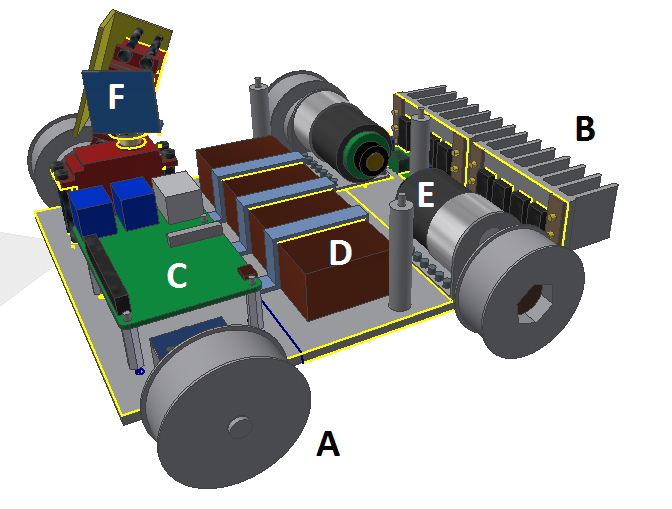
\includegraphics[scale=0.65]{imgs/calosc_2.png}
 	\caption[Model 3D projektowanego czołgu.]{\small{Model 3D projektowanego pojazdu. A - koła, B - mostki H wraz z radiatorami, C - Raspberry 2 Pi Model B, D - bateria, E - silniki prądu stałego, F - wieżyczka}}
	\label{mod3d}
    \end{center}
  \end{figure}
\namedsection{Podstawa pojazdu}
Wszystkie elementy zgrupowane na rysunku \ref{mod3d} tworzą korpus pojazdu, który został osadzony na sklejce brzozowej o grubości 5 mm. Materiał został wybrany pod kątem łatwości w obróbce oraz trwałości. Ze względu na jego warstwową strukturę jest on bardzo wytrzymały i jednocześnie bardzo lekki. Wyżej omówiony model pozwolił jednoznacznie dobrać wymiary podstawy oraz bardzo dokładnie wskazać miejsca, w których należało wykonać otwory mocujące dla poszczególnych komponentów. \newpage

  \begin{figure}[H]
    \begin{center}
      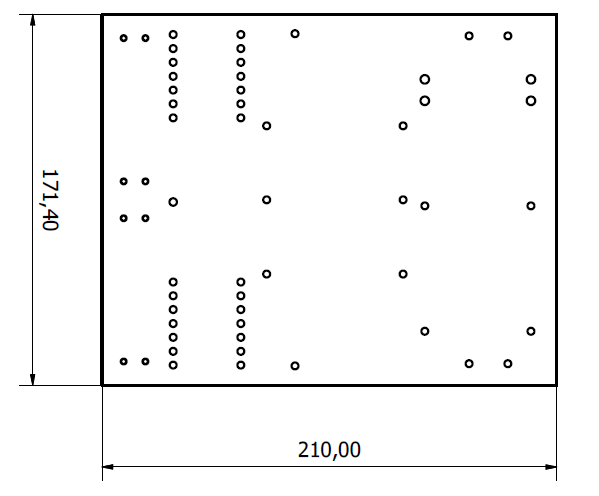
\includegraphics[scale=0.5]{imgs/podstawa.png}
 	\caption[Podstawa pojazdu.]{\small{Podstawa pojazdu wraz z naniesionymi wymiarami w milimetrach i otworami niezbędnymi do zamocowania poszczególnych elementów.}}
	\label{podst3d}
    \end{center}
  \end{figure}
\namedsection{Wieżyczka}
Wieża pojazdu zbudowana została w oparciu o 2 serwomechanizmy modelarskie TowerPro SG-5010. Są to zintegrowane układy elektroniczne zawierające sekcję mechaniczną (silnik wraz z przekładnią) oraz układ sterowania położeniem.
Na rysunku \ref{wieza3d} przedstawiono model omawianego segmentu. Serwomechanizm A jest zamocowany bezpośrednio do podstawy pojazdu i dzięki niemu realizowany jest obrót prawo/lewo wieży. Do orczyka, czyli obrotowej części mechanizmu, zamocowane zostało mocowanie serwomechanizmu B, które zostało wykonane z aluminiowego kątownika. Jest to materiał, który bardzo dobrze nadaje się do tego typu rozwiązań ponieważ jest tani, łatwo dostępny, lekki i stosunkowo wytrzymały.  

  \begin{figure}[H]
    \begin{center}
      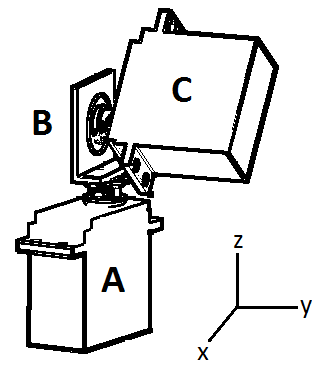
\includegraphics[scale=0.45]{imgs/wieza_3d.png}
 	\caption[Model wieżyczki.]{\small{Trójwymiarowy model konstrukcji wieżyczki robota. A - serwomechanizm odpowiedzialny za obrót wokół osi OZ, B - serwomechanizm obrotu w osi OY, C - łączenie pomiędzy elementami.}}
	\label{wieza3d}
    \end{center}
  \end{figure}
\namedsection{Napęd}
W projekcie wykorzystano dwa szczotkowe silniki prądu stałego Pololu 37Dx52L wraz z przekładnią 30:1. Dla napięcia 12 V pojedynczy silnik wytwarza moment obrotowy wynoszący 8 kg$\cdot$cm i obraca się z prędkością 350 obrotów na minutę. Rysunek techniczny przedstawiający dokładne wymiary wykorzystanego silnika przedstawiono na rysunku \ref{wymiary_silnika}. Maksymalny pobór prądu (przy zatrzymaniu wału) może wynieść około 5 A.

  \begin{figure}[H]
    \begin{center}
      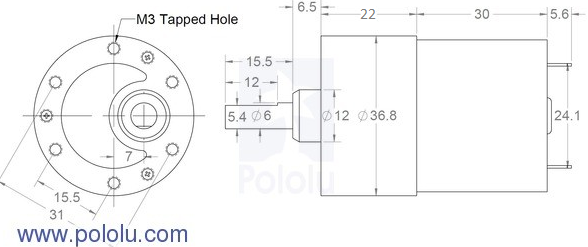
\includegraphics[scale=0.7]{imgs/silnik_wymiary.png}
 	\caption[Wymiary silnika Pololu 37Dx52L ]{\small{Wymiary wykorzystanego silnika - Pololu 37Dx52L }\footnotemark}
	\label{wymiary_silnika}
    \end{center}
  \end{figure}
  \footnotetext{http://pololu.com/, (data dostępu 20.10.2015r.)}

Jednym z założeń było zastosowanie w pojeździe napędu gąsienicowego. Robot zbudowany został w oparciu o 4 aluminiowe koła metryczne 27T5/32 - koła pasowe stosowane w przemyśle do przełożenia napędu. Ich średnica to 54 mm. Razem z dedykowanym pasem zębatym T5 o długości 420 mm tworzą układ gąsienic. Na ilustracji \ref{gasienice_elementy} przedstawione zostały wykorzystane elementy.

  \begin{figure}[H]
    \begin{center}
      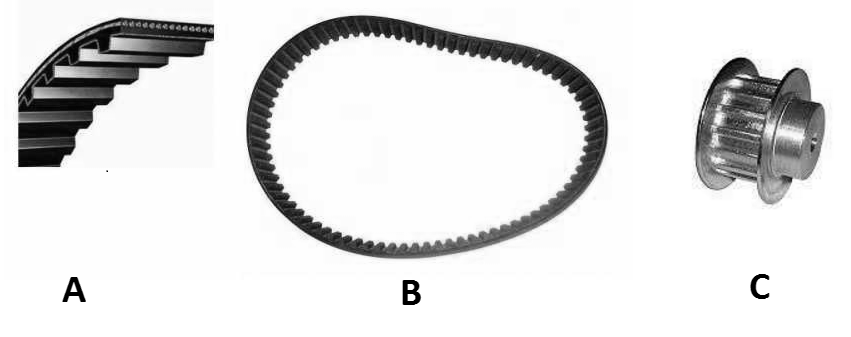
\includegraphics[scale=0.5]{imgs/gasienice.png}
 	\caption[Elementy gąsienic.]{\small{Rysunki A i B przedstawiają pas zębaty T5, C - koło zębate T5. }\footnotemark}
	\label{gasienice_elementy}
    \end{center}
  \end{figure}
  \footnotetext{http://centrum-cnc.pl/, (data dostępu 29.10.2015r.)}

Wybrane koła metryczne posiadały na środku otwór o średnicy 8 mm, podczas gdy oś silników ma średnicę 6 mm. Należało zatem wykonać mocowanie, pozwalające na sztywne osadzenie kół na wale. Do tego celu wykorzystano otrzymane wraz z silnikami sześciokątne nakładki, przedstawione na rysunku \ref{zamocowanie_szesciokatne}. Wycięcie otworu w kształcie sześciokąta w warunkach domowych jest bardzo trudne. W związku z tym, dzięki projektowi w środowisku CAD, możliwe było zlecenie wykonania go firmie zewnętrznej, specjalizującej się w cięciu wodą pod wysokim ciśnieniem.
\newpage
  \begin{figure}[H]
    \begin{center}
      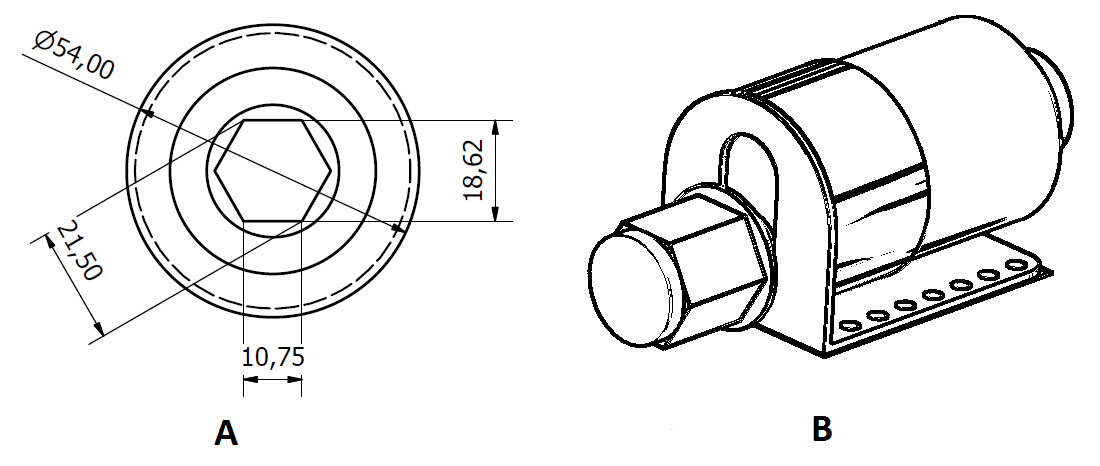
\includegraphics[scale=0.40]{imgs/moc_kol_tyl.png}
 	\caption[Model tylnych kół.]{\small{Na ilustracji znajduje się rysunek techniczny koła metrycznego(A) dostosowanego na potrzeby mocowania na silniku z wykorzystaniem sześciokątnej przejściówki(B).}}
	\label{zamocowanie_szesciokatne}
    \end{center}
  \end{figure}

Podczas tworzenia projektu należało także rozważyć sposób mocowania przednich kół. Ze względu na fakt, iż gąsienice (prawa/lewa) mogą obracać się jednocześnie w dwóch rożnych kierunkach, należało zastosować osobną oś dla prawego oraz lewego koła. Jej model przedstawiony został na rysunku \ref{zamocowanie_przod}. Element A wykonany został z drewna dębowego, które jest bardzo twarde i pozwala na dokładne spasowanie z osią B, wykonaną z aluminium.

  \begin{figure}[H]
    \begin{center}
      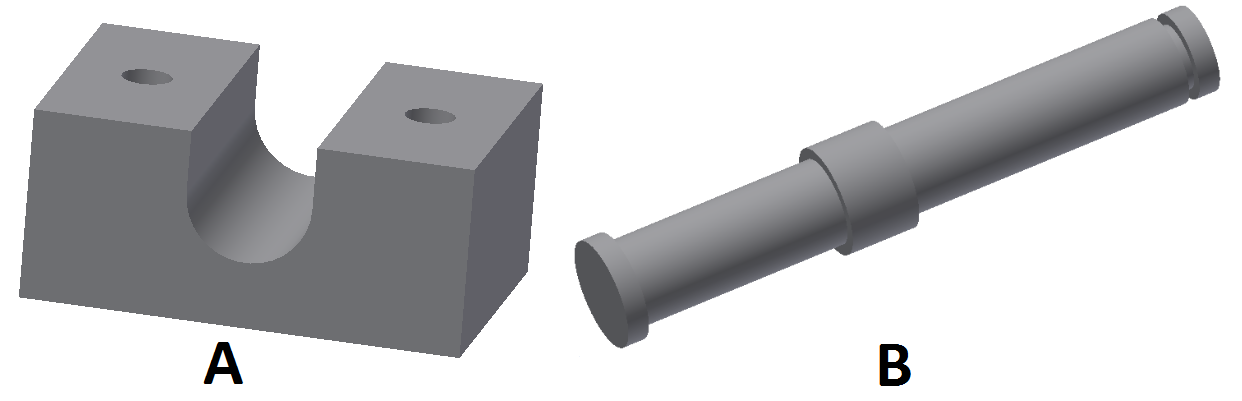
\includegraphics[scale=0.40]{imgs/moc_kol_prz.png}
 	\caption[Model mocowania kół przednich.]{\small{Na rysunku przedstawiony został model mocowań kół przednich pojazdu. A - przedstawia blok łączący oś B z podstawą robota.}}
	\label{zamocowanie_przod}
    \end{center}
  \end{figure}
\namedsection{Efekt końcowy}
Wykonanie oraz ostateczne dopasowanie wszystkich elementów było dość czasochłonne. Należy jednak wspomnieć o tym, że dzięki wykonaniu trójwymiarowego modelu czas ten niewątpliwie uległ znacznemu skróceniu. Końcowy efekt, wraz z zamocowaniem części elektronicznej przedstawiony został na zdjęciu poniżej (rys. \ref{czolg_calosc}).
\newpage
  \begin{figure}[H]
    \begin{center}
      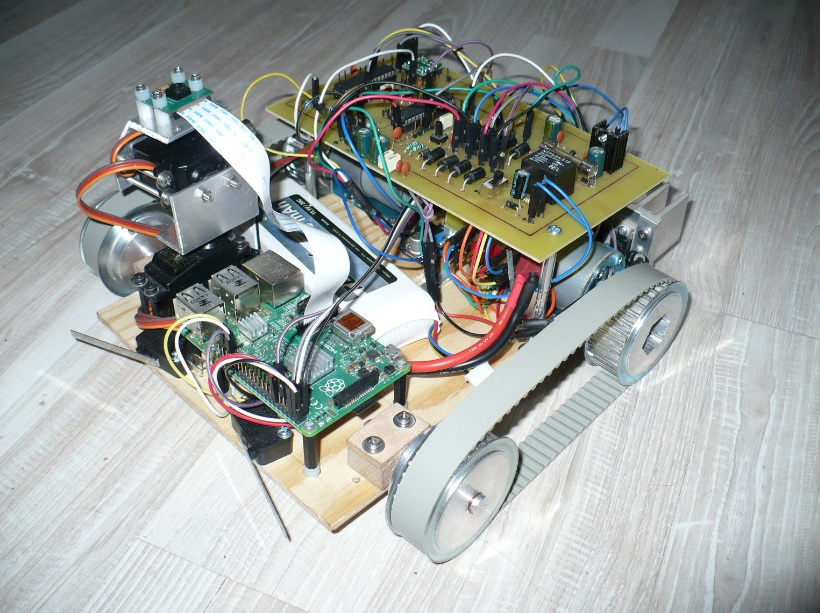
\includegraphics[scale=0.65]{imgs/czolg2.jpg}
 	\caption[Zbudowany model.]{\small{Zdjęcie przedstawia kompletny robot typu czołg. Jest to całkowicie wykonany model wraz z częścią elektroniczną.}}
	\label{czolg_calosc}
    \end{center}
  \end{figure}
